\documentclass[11pt,aspectratio=169]{beamer}
\usetheme{Madrid}

% ======================= PACKAGES =======================
\usepackage{graphicx}
\usepackage{booktabs}
\usepackage{adjustbox}
\usepackage{multicol}
\usepackage{amsmath}
\usepackage{amssymb}
\usepackage{tikz}
\usetikzlibrary{arrows,shapes,positioning,shadows,trees}
\usepackage{listings}
\usepackage{xcolor}

% ======================= COLOR DEFINITIONS =======================
% Primary color scheme: Blue/Teal for Digital Finance
\definecolor{dfblue}{RGB}{0,102,204}
\definecolor{dfteal}{RGB}{0,153,153}
\definecolor{dfcyan}{RGB}{51,187,204}
\definecolor{dflightblue}{RGB}{153,204,255}
\definecolor{dflightblue2}{RGB}{173,214,255}
\definecolor{dflightblue3}{RGB}{193,224,255}
\definecolor{dflightblue4}{RGB}{213,234,255}

% Accent colors for finance applications
\definecolor{dfgreen}{RGB}{44, 160, 44}
\definecolor{dfred}{RGB}{214, 39, 40}
\definecolor{dforange}{RGB}{255, 127, 14}
\definecolor{dfgray}{RGB}{127, 127, 127}

% Utility colors
\definecolor{lightgray}{RGB}{240, 240, 240}
\definecolor{midgray}{RGB}{180, 180, 180}
\definecolor{codebg}{RGB}{245, 245, 245}

% ======================= THEME CUSTOMIZATION =======================
% Apply Digital Finance color scheme to Madrid theme
\setbeamercolor{palette primary}{bg=dflightblue3,fg=dfblue}
\setbeamercolor{palette secondary}{bg=dflightblue2,fg=dfblue}
\setbeamercolor{palette tertiary}{bg=dfteal,fg=white}
\setbeamercolor{palette quaternary}{bg=dfblue,fg=white}

\setbeamercolor{structure}{fg=dfblue}
\setbeamercolor{section in toc}{fg=dfblue}
\setbeamercolor{subsection in toc}{fg=dfteal}
\setbeamercolor{title}{fg=dfblue}
\setbeamercolor{frametitle}{fg=dfblue,bg=dflightblue3}
\setbeamercolor{block title}{bg=dflightblue2,fg=dfblue}
\setbeamercolor{block body}{bg=dflightblue4,fg=black}

% Remove navigation symbols for cleaner look
\setbeamertemplate{navigation symbols}{}

% Clean itemize/enumerate
\setbeamertemplate{itemize items}[circle]
\setbeamertemplate{enumerate items}[default]

% Margins for readability
\setbeamersize{text margin left=8mm,text margin right=8mm}

% ======================= LISTINGS CONFIGURATION =======================
% Python code style
\lstdefinestyle{pythonstyle}{
    language=Python,
    basicstyle=\ttfamily\footnotesize,
    keywordstyle=\color{dfblue}\bfseries,
    stringstyle=\color{dforange},
    commentstyle=\color{dfgray}\itshape,
    numberstyle=\tiny\color{dfgray},
    numbers=left,
    numbersep=5pt,
    backgroundcolor=\color{codebg},
    showspaces=false,
    showstringspaces=false,
    showtabs=false,
    frame=single,
    rulecolor=\color{midgray},
    tabsize=4,
    captionpos=b,
    breaklines=true,
    breakatwhitespace=false,
    escapeinside={(*@}{@*)},
    xleftmargin=10pt,
    xrightmargin=10pt
}

% Solidity code style
\lstdefinestyle{soliditystyle}{
    language=Java, % closest approximation
    basicstyle=\ttfamily\footnotesize,
    keywordstyle=\color{dfteal}\bfseries,
    stringstyle=\color{dforange},
    commentstyle=\color{dfgray}\itshape,
    numberstyle=\tiny\color{dfgray},
    numbers=left,
    numbersep=5pt,
    backgroundcolor=\color{codebg},
    showspaces=false,
    showstringspaces=false,
    showtabs=false,
    frame=single,
    rulecolor=\color{midgray},
    tabsize=2,
    captionpos=b,
    breaklines=true,
    breakatwhitespace=false,
    escapeinside={(*@}{@*)},
    xleftmargin=10pt,
    xrightmargin=10pt,
    morekeywords={pragma, contract, function, returns, public, private, view, pure, payable, address, uint256, mapping, event, modifier}
}

% Inline code command
\newcommand{\code}[1]{\texttt{\color{dfblue}#1}}

% ======================= CUSTOM COMMANDS =======================
% Bottom annotation (Madrid-style)
\newcommand{\bottomnote}[1]{%
\vfill
\vspace{-2mm}
\textcolor{dflightblue2}{\rule{\textwidth}{0.4pt}}
\vspace{1mm}
\footnotesize
\textbf{#1}
}

% Compact list spacing
\newcommand{\compactlist}{%
\setlength{\itemsep}{0pt}%
\setlength{\parskip}{0pt}%
\setlength{\parsep}{0pt}%
}

% Chart placeholder
\newcommand{\chartplaceholder}[2][5cm]{%
\begin{center}
\begin{adjustbox}{max width=0.95\textwidth, max height=#1}
\framebox[\textwidth][c]{%
\rule{0pt}{#1}%
\textcolor{midgray}{[#2]}%
}
\end{adjustbox}
\end{center}
}

% ======================= FINANCE NOTATION MACROS =======================
% Probability and statistics
\newcommand{\E}{\mathbb{E}} % Expected value
\newcommand{\Var}{\mathrm{Var}} % Variance
\newcommand{\Cov}{\mathrm{Cov}} % Covariance
\newcommand{\Prob}{\mathbb{P}} % Probability

% Distributions
\newcommand{\Normal}{\mathcal{N}} % Normal distribution
\newcommand{\Uniform}{\mathcal{U}} % Uniform distribution

% Returns and prices
\newcommand{\Ret}{R} % Return
\newcommand{\LogRet}{r} % Log return
\newcommand{\Price}{S} % Price/Stock price
\newcommand{\Strike}{K} % Strike price

% Options and derivatives
\newcommand{\CallPrice}{C} % Call option price
\newcommand{\PutPrice}{P} % Put option price
\newcommand{\Greeks}[1]{\mathit{#1}} % Greek letters

% Risk measures
\newcommand{\VaR}{\mathrm{VaR}} % Value at Risk
\newcommand{\CVaR}{\mathrm{CVaR}} % Conditional VaR
\newcommand{\Sharpe}{\mathrm{SR}} % Sharpe Ratio

% Time series
\newcommand{\AR}{\mathrm{AR}} % Autoregressive
\newcommand{\MA}{\mathrm{MA}} % Moving average
\newcommand{\GARCH}{\mathrm{GARCH}} % GARCH

% Blockchain/Crypto
\newcommand{\Hash}{\mathrm{Hash}} % Hash function
\newcommand{\Block}{\mathcal{B}} % Block
\newcommand{\Chain}{\mathcal{C}} % Chain

% Real numbers, integers
\newcommand{\R}{\mathbb{R}}
\newcommand{\Z}{\mathbb{Z}}
\newcommand{\N}{\mathbb{N}}

% ======================= TIKZ STYLES =======================
% Styles for finance-related diagrams
\tikzstyle{process} = [rectangle, minimum width=3cm, minimum height=1cm, text centered, draw=dfblue, fill=dflightblue4, thick]
\tikzstyle{decision} = [diamond, minimum width=3cm, minimum height=1cm, text centered, draw=dfteal, fill=dflightblue4, thick]
\tikzstyle{arrow} = [thick,->,>=stealth,color=dfblue]
\tikzstyle{blockchain} = [rectangle, rounded corners, minimum width=2.5cm, minimum height=1cm, text centered, draw=dfteal, fill=dflightblue3, thick]
\tikzstyle{transaction} = [circle, minimum size=0.8cm, text centered, draw=dforange, fill=dflightblue4, thick]

% ======================= FOOTER TEMPLATE =======================
\setbeamertemplate{footline}{
    \hbox{\begin{beamercolorbox}[wd=\paperwidth,ht=2.5ex,dp=1ex,leftskip=.5em,rightskip=.5em]{author in head/foot}
    \tiny
    \textbf{Digital Finance} \hfill
    Joerg Osterrieder \hfill
    \insertdate \hfill
    Page \insertframenumber{} / \inserttotalframenumber
    \end{beamercolorbox}}
}

% ======================= SECTION DIVIDER TEMPLATE =======================
\AtBeginSection[]{
\begin{frame}[plain]
\vfill
\centering
\begin{beamercolorbox}[sep=12pt,center]{title}
\usebeamerfont{title}\LARGE\insertsection\par
\end{beamercolorbox}
\vfill
\end{frame}
}


% ======================= DOCUMENT INFO =======================
\title{Topic 2.2: The API Economy and Banking-as-a-Service}
\subtitle{How Non-Banks Offer Financial Services}
\author{Joerg Osterrieder}
\institute{Digital Finance}
\date{Digital Finance}

\begin{document}

% ============================================================================
% SLIDE 1: TITLE
% ============================================================================
\begin{frame}[plain]
\titlepage
\end{frame}

% ============================================================================
% SLIDE 2: LEARNING OBJECTIVES
% ============================================================================
\begin{frame}{Learning Objectives}
\begin{block}{By the end of this topic, you will be able to:}
\begin{enumerate}
\item \textbf{Define} what an API is and explain why it matters for modern finance
\item \textbf{Explain} how open banking regulation enables third-party access to banking data
\item \textbf{Describe} the Banking-as-a-Service model and how it separates licenses from experiences
\item \textbf{Analyze} how embedded finance allows non-banks to offer financial products
\item \textbf{Compare} token-based security with traditional password sharing
\item \textbf{Apply} open banking concepts through API simulation exercises (NB03)
\end{enumerate}
\end{block}

\vspace{3mm}
\textbf{Key Competency}: Explain how APIs, open banking, and BaaS work together to let any company offer financial services --- and identify the risks involved.
\end{frame}

% ============================================================================
% SLIDE 3: PREREQUISITES
% ============================================================================
\begin{frame}{Prerequisites: What You Need to Know}
\begin{columns}[T]
\begin{column}{0.5\textwidth}
\textbf{No Prior Technical Knowledge Required}

This topic is self-contained. We will explain:
\begin{itemize}
\item How software systems communicate with each other
\item What it means to authenticate and authorize
\item How data flows between a bank and a third party
\item Why regulation matters for innovation
\end{itemize}
\end{column}
\begin{column}{0.5\textwidth}
\begin{block}{Key Background Concepts}
\begin{itemize}
\item \textbf{Client-Server}: One system requests, another responds
\item \textbf{Internet Protocol}: Rules for data transmission
\item \textbf{Authentication}: Proving \textit{who} you are
\item \textbf{Authorization}: Defining \textit{what} you are allowed to do
\end{itemize}
\end{block}
\end{column}
\end{columns}

\vspace{3mm}
\begin{alertblock}{From Topic 2.1}
Recall: Banks have traditionally been ``bundled'' --- offering all services under one roof. This topic explains \textit{how} APIs enable ``unbundling.''
\end{alertblock}
\end{frame}

% ============================================================================
% SLIDE 4: THE TRADITIONAL BANKING PROBLEM
% ============================================================================
\begin{frame}{The Traditional Banking Problem}
\begin{alertblock}{The Problem}
Banks built closed, proprietary systems for decades. How could a startup innovate on top of banking infrastructure it could not access?
\end{alertblock}

\vspace{3mm}
\begin{center}
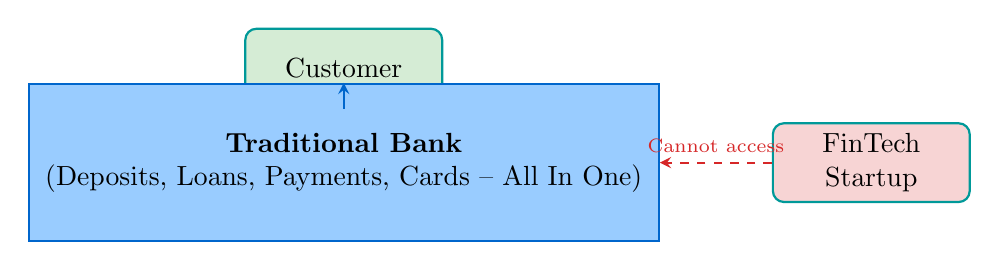
\begin{tikzpicture}[node distance=1.2cm]
% Traditional model
\node (cust) [blockchain, fill=dfgreen!20] {Customer};
\node (bank) [process, below of=cust, minimum width=8cm, minimum height=2cm, fill=dflightblue] {};
\node at (bank.center) [align=center] {\textbf{Traditional Bank}\\(Deposits, Loans, Payments, Cards -- All In One)};
\node (fintech) [blockchain, right of=bank, xshift=5.5cm, fill=dfred!20, align=center] {FinTech\\Startup};

% Problem arrows
\draw[arrow, dashed, color=dfred] (fintech) -- node[above, font=\scriptsize] {Cannot access} (bank);
\draw[arrow] (cust) -- (bank);
\end{tikzpicture}
\end{center}
\end{frame}

% ~~~~~~~~~~~~~~~~~~~~~~~~~~~~~~~~~~~~~~~~~~~~~~~~~~~~~~~~~~~~~~~~~~~~~~~~~~~~
\begin{frame}{The Traditional Banking Problem (cont.)}
\textbf{The Concept:}
\begin{itemize}
\item \textbf{Closed Systems}: Each bank built its own proprietary technology
\item \textbf{No Standard Communication}: No common language between institutions
\item \textbf{Barrier to Innovation}: Startups could not build on banking infrastructure
\item \textbf{Customer Lock-in}: Switching providers meant starting from scratch
\end{itemize}

\vspace{2mm}
\begin{block}{The Insight}
The solution is \textcolor{dfblue}{Application Programming Interfaces (APIs)} --- standardized contracts that let any authorized software talk to bank systems.
\end{block}
\end{frame}

% ============================================================================
% SLIDE 5: WHAT IS AN API?
% ============================================================================
\begin{frame}{What is an API?}
\begin{alertblock}{The Problem}
How do different software systems talk to each other without knowing each other's internal workings?
\end{alertblock}

\vspace{3mm}
\begin{columns}[T]
\begin{column}{0.5\textwidth}
\textbf{Non-Technical Definition:}
\begin{itemize}
\item An API is a \textbf{contract} between software systems
\item It defines what you can \textbf{request} and what you will \textbf{receive}
\item Think of it like a restaurant menu: a fixed set of options, in a standardized format
\end{itemize}

\vspace{3mm}
\footnotesize{\textcolor{dfteal}{\textbf{Jargon explained:}} \textit{API} stands for Application Programming Interface. \textit{Endpoint} = a specific address where you send requests (like a phone number). \textit{Request} = asking for data. \textit{Response} = the data you get back.}
\end{column}
\begin{column}{0.5\textwidth}
\begin{block}{Why APIs Matter for Finance}
\begin{itemize}
\item \textbf{Unbundling}: Break a monolithic bank into separate, accessible components
\item \textbf{Speed}: Integrate with banking infrastructure quickly instead of building from scratch
\item \textbf{Innovation}: Any authorized developer can access banking capabilities
\item \textbf{Competition}: A more level playing field between incumbents and startups
\end{itemize}
\end{block}
\end{column}
\end{columns}

\vspace{2mm}
\begin{block}{The Insight}
APIs let any developer access banking capabilities without building them --- just as a restaurant menu lets you order food without knowing how to cook.
\end{block}
\end{frame}

% ============================================================================
% SLIDE 6: THE RESTAURANT ANALOGY
% ============================================================================
\begin{frame}{The Restaurant Analogy}
\begin{center}
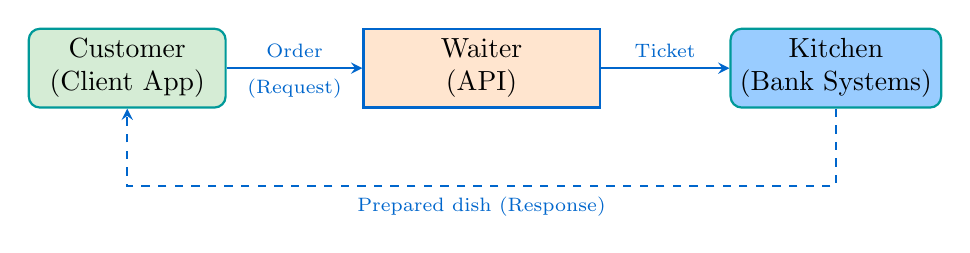
\begin{tikzpicture}[node distance=2cm]
% Customer
\node (customer) [blockchain, fill=dfgreen!20, align=center] {Customer\\(Client App)};

% Waiter
\node (waiter) [process, right of=customer, xshift=2.5cm, fill=dforange!20, align=center] {Waiter\\(API)};

% Kitchen
\node (kitchen) [blockchain, right of=waiter, xshift=2.5cm, fill=dflightblue, align=center] {Kitchen\\(Bank Systems)};

% Arrows
\draw[arrow] (customer) -- node[above, font=\scriptsize] {Order} node[below, font=\scriptsize] {(Request)} (waiter);
\draw[arrow] (waiter) -- node[above, font=\scriptsize] {Ticket} (kitchen);
\draw[arrow, dashed] (kitchen) -- ++(0,-1.5) -| node[below, pos=0.25, font=\scriptsize] {Prepared dish (Response)} (customer);
\end{tikzpicture}
\end{center}

\vspace{3mm}
\begin{columns}[T]
\begin{column}{0.33\textwidth}
\textbf{The Menu (API Spec)}
\begin{itemize}
\item Lists available options
\item Standardized formats
\item Clear descriptions of what you can order
\end{itemize}
\end{column}
\begin{column}{0.33\textwidth}
\textbf{The Waiter (API)}
\begin{itemize}
\item Takes your request
\item Validates the order
\item Returns the result
\end{itemize}
\end{column}
\begin{column}{0.33\textwidth}
\textbf{The Kitchen (Bank)}
\begin{itemize}
\item Does the actual work
\item Hidden from the customer
\item Can change internally without affecting the menu
\end{itemize}
\end{column}
\end{columns}

\vspace{3mm}
\textbf{Key takeaway}: You do not need to know how the kitchen works. You just need to know the menu.
\end{frame}

% ============================================================================
% SLIDE 7: HOW APIs COMMUNICATE
% ============================================================================
\begin{frame}[fragile]{How APIs Communicate}
\begin{alertblock}{The Problem}
What does an API request actually look like? How does a FinTech app ``talk'' to a bank?
\end{alertblock}

\vspace{3mm}
\begin{columns}[T]
\begin{column}{0.5\textwidth}
\textbf{Four Core Operations:}
\begin{itemize}
\item \textbf{GET}: Read information\\
  {\scriptsize (``Show me my account balance'')}
\item \textbf{POST}: Create or send something\\
  {\scriptsize (``Send a payment to Alice'')}
\item \textbf{PUT}: Update existing information\\
  {\scriptsize (``Change my address'')}
\item \textbf{DELETE}: Remove something\\
  {\scriptsize (``Cancel a pending transfer'')}
\end{itemize}
\end{column}
\begin{column}{0.5\textwidth}
\textbf{Simplified Example:}
\begin{lstlisting}[style=pythonstyle, basicstyle=\ttfamily\scriptsize]
# Read account balance
GET /accounts/balance

# Send a payment
POST /payments
{
  "recipient": "Alice",
  "amount": "lunch money"
}
\end{lstlisting}
\end{column}
\end{columns}

\vspace{3mm}
\begin{block}{The Insight}
These four operations --- read, create, update, delete --- cover nearly everything a financial application needs to do. The simplicity of this contract is what makes APIs so powerful.
\end{block}

\vspace{2mm}
\footnotesize{\textcolor{dfteal}{\textbf{Jargon explained:}} \textit{HTTP} is the language computers use to communicate on the web. Every time you load a webpage, your browser sends HTTP requests.}
\end{frame}

% ============================================================================
% SLIDE 8: THE UNBUNDLING OF BANKING
% ============================================================================
\begin{frame}{The Unbundling of Banking}
\begin{alertblock}{The Problem}
What happens when you break a monolithic bank into separate, independently accessible services?
\end{alertblock}

\vspace{3mm}
\begin{center}
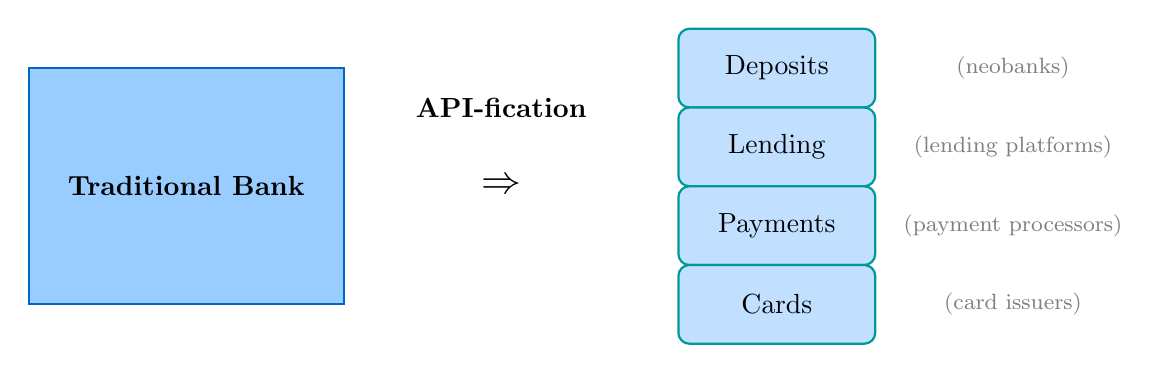
\begin{tikzpicture}[node distance=1.5cm]
% Traditional bank
\node (bank) [process, minimum width=4cm, minimum height=3cm, fill=dflightblue] {};
\node at (bank.center) {\textbf{Traditional Bank}};

% Arrow
\node (arw) [right of=bank, xshift=2.5cm] {\Large$\Rightarrow$};
\node[above of=arw, yshift=-0.5cm] {\textbf{API-fication}};

% Unbundled services
\node (deposits) [blockchain, right of=arw, xshift=2cm, yshift=1.5cm] {Deposits};
\node (loans) [blockchain, right of=arw, xshift=2cm, yshift=0.5cm] {Lending};
\node (payments) [blockchain, right of=arw, xshift=2cm, yshift=-0.5cm] {Payments};
\node (cards) [blockchain, right of=arw, xshift=2cm, yshift=-1.5cm] {Cards};

% Generic labels (no company names)
\node[right of=deposits, xshift=1.5cm, font=\footnotesize, text=dfgray] {(neobanks)};
\node[right of=loans, xshift=1.5cm, font=\footnotesize, text=dfgray] {(lending platforms)};
\node[right of=payments, xshift=1.5cm, font=\footnotesize, text=dfgray] {(payment processors)};
\node[right of=cards, xshift=1.5cm, font=\footnotesize, text=dfgray] {(card issuers)};
\end{tikzpicture}
\end{center}
\end{frame}

% ~~~~~~~~~~~~~~~~~~~~~~~~~~~~~~~~~~~~~~~~~~~~~~~~~~~~~~~~~~~~~~~~~~~~~~~~~~~~
\begin{frame}{The Unbundling of Banking (cont.)}
\textbf{The Concept:}
\begin{itemize}
\item Each banking function becomes a standalone service accessible via API
\item Different companies can specialize in one service and do it exceptionally well
\item A single startup can compete with a bank on one specific dimension
\end{itemize}

\vspace{2mm}
\begin{block}{The Insight}
Any service can now be offered independently by a different company. The ``bank'' is no longer a single institution --- it is a collection of components that can be mixed and matched.
\end{block}
\end{frame}

% ============================================================================
% SLIDE 9: OPEN BANKING -- THE CONCEPT
% ============================================================================
\begin{frame}{Open Banking: The Concept}
\begin{alertblock}{The Problem}
Why would banks voluntarily share your data with competitors? Most would not --- unless regulators require it.
\end{alertblock}

\vspace{3mm}
\begin{block}{Definition}
\textbf{Open Banking} is a regulatory and technical framework in which banks provide third-party financial service providers access to consumer banking data and payment functionality through secure APIs --- \textit{with customer consent}.
\end{block}

\vspace{3mm}
\begin{columns}[T]
\begin{column}{0.5\textwidth}
\textbf{What Banks Must Share (with consent):}
\begin{itemize}
\item Account balances
\item Transaction history
\item Payment initiation capability
\item Account holder information
\end{itemize}
\end{column}
\begin{column}{0.5\textwidth}
\textbf{Key Principles:}
\begin{itemize}
\item \textbf{Customer Control}: You decide who sees your data
\item \textbf{Standardized}: Same format across all banks
\item \textbf{Secure}: Strong authentication required
\item \textbf{Regulated}: Government oversight ensures compliance
\end{itemize}
\end{column}
\end{columns}

\vspace{3mm}
\begin{block}{The Insight}
Open banking shifts power from banks to consumers. Your financial data belongs to \textit{you}, not to your bank.
\end{block}
\end{frame}

% ============================================================================
% SLIDE 10: OPEN BANKING REGULATION
% ============================================================================
\begin{frame}{Open Banking: Regulatory Approaches}
\begin{alertblock}{The Problem}
How do different regions approach opening up banking data --- and why does the approach matter?
\end{alertblock}

\vspace{3mm}
\begin{columns}[T]
\begin{column}{0.5\textwidth}
\textbf{Regulated Approach:}
\begin{itemize}
\item Governments \textbf{mandate} that banks provide APIs
\item Standardized specifications ensure interoperability
\item Third parties must be licensed and supervised
\item Adopted by several European and Asia-Pacific jurisdictions
\end{itemize}

\vspace{2mm}
\textit{``Banks must open up --- whether they want to or not.''}
\end{column}
\begin{column}{0.5\textwidth}
\textbf{Market-Driven Approach:}
\begin{itemize}
\item No government mandate for standardized APIs
\item Data aggregators negotiate access with banks individually
\item Screen-scraping (sharing passwords) remains common
\item Innovation happens, but without standardization
\end{itemize}

\vspace{2mm}
\textit{``Let the market figure it out.''}
\end{column}
\end{columns}

\vspace{4mm}
\begin{block}{The Insight}
The regulatory approach shapes how fast innovation happens. Mandated standards create a level playing field quickly; market-driven approaches allow flexibility but create fragmentation.
\end{block}
\end{frame}

% ============================================================================
% SLIDE 11: AISP AND PISP
% ============================================================================
\begin{frame}{AISP and PISP: Read Access vs.\ Write Access}
\begin{alertblock}{The Problem}
What can third parties actually \textit{do} with your banking data --- and how is this regulated?
\end{alertblock}

\vspace{3mm}
\begin{columns}[T]
\begin{column}{0.48\textwidth}
\begin{block}{AISP --- Account Information}
\textbf{Account Information Service Provider}
\vspace{2mm}
\begin{itemize}\compactlist
\item \textbf{What}: Reads your account data
\item \textbf{Use cases}:
  \begin{itemize}\compactlist
  \item Budgeting apps that show all your accounts in one place
  \item Credit assessment based on transaction history
  \item Financial planning tools
  \end{itemize}
\item \textbf{Permission}: \textcolor{dfgreen}{Read-only access}
\end{itemize}
\end{block}
\end{column}
\begin{column}{0.48\textwidth}
\begin{block}{PISP --- Payment Initiation}
\textbf{Payment Initiation Service Provider}
\vspace{2mm}
\begin{itemize}\compactlist
\item \textbf{What}: Initiates payments from your account
\item \textbf{Use cases}:
  \begin{itemize}\compactlist
  \item E-commerce checkout directly from your bank
  \item Bill payment services
  \item Money transfer apps
  \end{itemize}
\item \textbf{Permission}: \textcolor{dforange}{Write access (with explicit approval)}
\end{itemize}
\end{block}
\end{column}
\end{columns}
\end{frame}

% ~~~~~~~~~~~~~~~~~~~~~~~~~~~~~~~~~~~~~~~~~~~~~~~~~~~~~~~~~~~~~~~~~~~~~~~~~~~~
\begin{frame}{AISP and PISP: Read Access vs.\ Write Access (cont.)}
\begin{block}{The Insight}
Read access and write access are regulated differently because the risks differ. Seeing your balance is far less risky than moving your money.
\end{block}

\vspace{2mm}
\footnotesize{\textcolor{dfteal}{\textbf{Jargon explained:}} \textit{TPP (Third Party Provider)} = a company (not your bank) that accesses your bank data with your permission. \textit{Account aggregation} = combining data from multiple banks into one view.}
\end{frame}

% ============================================================================
% SLIDE 12: OPEN BANKING ARCHITECTURE
% ============================================================================
\begin{frame}{Open Banking Architecture: The Consent Flow}
\begin{alertblock}{The Problem}
How does the consent flow actually work --- and how is your data kept secure?
\end{alertblock}

\vspace{1mm}
\begin{center}
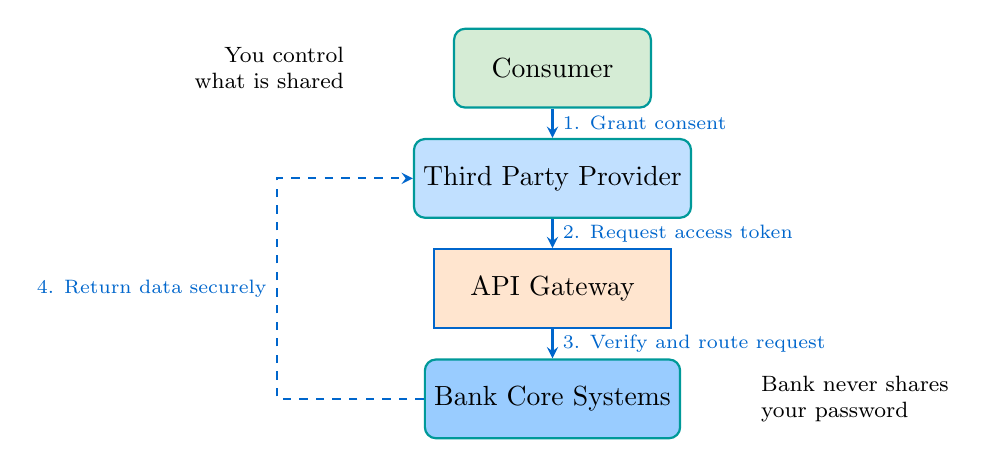
\begin{tikzpicture}[node distance=1.4cm]
% Layers
\node (consumer) [blockchain, fill=dfgreen!20] {Consumer};
\node (tpp) [blockchain, below of=consumer] {Third Party Provider};
\node (api) [process, below of=tpp, fill=dforange!20] {API Gateway};
\node (bank) [blockchain, below of=api, fill=dflightblue] {Bank Core Systems};

% Arrows with consent flow
\draw[arrow] (consumer) -- node[right, font=\scriptsize] {1. Grant consent} (tpp);
\draw[arrow] (tpp) -- node[right, font=\scriptsize] {2. Request access token} (api);
\draw[arrow] (api) -- node[right, font=\scriptsize] {3. Verify and route request} (bank);
\draw[arrow, dashed] (bank) -- ++(-3.5,0) |- node[left, pos=0.25, font=\scriptsize] {4. Return data securely} (tpp);

% Side labels
\node[left of=consumer, xshift=-2.5cm, text width=2.5cm, font=\footnotesize, align=right] {You control\\what is shared};
\node[right of=bank, xshift=2.5cm, text width=2.5cm, font=\footnotesize, align=left] {Bank never shares\\your password};
\end{tikzpicture}
\end{center}
\end{frame}

% ~~~~~~~~~~~~~~~~~~~~~~~~~~~~~~~~~~~~~~~~~~~~~~~~~~~~~~~~~~~~~~~~~~~~~~~~~~~~
\begin{frame}{Open Banking Architecture: The Consent Flow (cont.)}
\begin{block}{The Insight}
You never share your password with the third party. Instead, the bank issues a temporary \textit{token} --- like a concert wristband that grants limited access and can be revoked at any time.
\end{block}
\end{frame}

% ============================================================================
% SLIDE 13: API TYPES IN FINANCIAL SERVICES
% ============================================================================
\begin{frame}{API Types in Financial Services}
\begin{alertblock}{The Problem}
What financial services can be accessed via API --- and what does each one do?
\end{alertblock}

\vspace{3mm}
\begin{center}
\begin{tabular}{p{3.2cm}p{5cm}p{3.5cm}}
\toprule
\textbf{API Type} & \textbf{Function} & \textbf{Who Uses It} \\
\midrule
\textbf{Account Information} & Read balances, transaction history & Budgeting apps, lenders \\
\textbf{Payment Initiation} & Trigger bank-to-bank transfers & E-commerce, bill pay \\
\textbf{Card Issuance} & Create virtual or physical cards & Neobanks, expense tools \\
\textbf{Lending} & Originate and service loans & Lending platforms \\
\textbf{Identity / KYC} & Verify a customer's identity & Any regulated service \\
\textbf{Core Banking} & Full account ledger functionality & Companies building banks \\
\bottomrule
\end{tabular}
\end{center}

\vspace{4mm}
\begin{block}{The Insight}
You can assemble a ``bank'' from API building blocks without building any of the underlying infrastructure yourself. This is the foundation of Banking-as-a-Service.
\end{block}

\vspace{2mm}
\footnotesize{\textcolor{dfteal}{\textbf{Jargon explained:}} \textit{KYC} = Know Your Customer, the process of verifying someone's identity before providing financial services. Required by law in most countries.}
\end{frame}

% ============================================================================
% SLIDE 14: BANKING-AS-A-SERVICE: THE CONCEPT
% ============================================================================
\begin{frame}{Banking-as-a-Service: The Concept}
\begin{alertblock}{The Problem}
What if you want to offer banking products to your customers --- but you do not want to become a bank?
\end{alertblock}

\vspace{3mm}
\begin{block}{Definition}
\textbf{Banking-as-a-Service (BaaS)} is a model where licensed banks provide their banking infrastructure --- including their charter, compliance systems, and account ledger --- to non-banks via APIs, enabling them to offer financial products under their own brand.
\end{block}

\vspace{3mm}
\begin{columns}[T]
\begin{column}{0.48\textwidth}
\textbf{Without BaaS:}
\begin{itemize}\compactlist
\item Obtaining a banking license requires enormous capital and years of effort
\item Must build compliance infrastructure from scratch
\item Need to hire regulatory and legal experts
\item Must create core banking systems
\end{itemize}
\end{column}
\begin{column}{0.48\textwidth}
\textbf{With BaaS:}
\begin{itemize}\compactlist
\item ``Rent'' a license from a partner bank
\item Use pre-built compliance tools
\item Focus entirely on customer experience
\item Launch much faster than building a bank
\end{itemize}
\end{column}
\end{columns}
\end{frame}

% ~~~~~~~~~~~~~~~~~~~~~~~~~~~~~~~~~~~~~~~~~~~~~~~~~~~~~~~~~~~~~~~~~~~~~~~~~~~~
\begin{frame}{Banking-as-a-Service: The Concept (cont.)}
\begin{block}{The Insight}
BaaS separates ``who builds the experience'' from ``who holds the license.'' This is what allows technology companies to offer bank accounts, cards, and loans.
\end{block}
\end{frame}

% ============================================================================
% SLIDE 15: THE BaaS STACK
% ============================================================================
\begin{frame}{The BaaS Stack: What You Build vs.\ What You Rent}
\begin{alertblock}{The Problem}
In a BaaS arrangement, what does the FinTech actually build --- and what does it rent from others?
\end{alertblock}

\vspace{3mm}
\begin{center}
\begin{adjustbox}{max width=\textwidth}
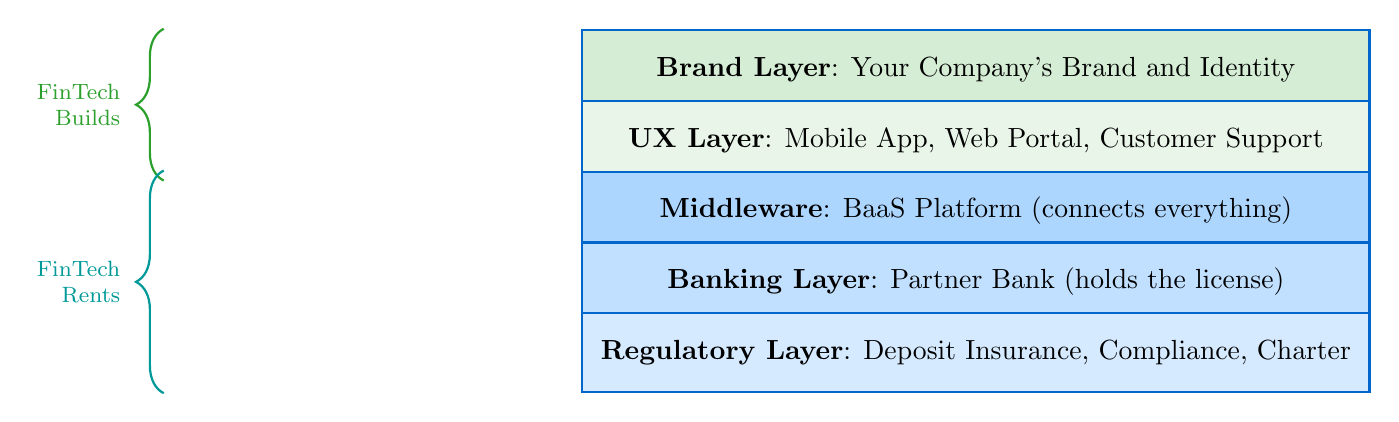
\begin{tikzpicture}[node distance=0.9cm]
% Stack
\node (brand) [process, minimum width=10cm, fill=dfgreen!20] {\textbf{Brand Layer}: Your Company's Brand and Identity};
\node (ux) [process, minimum width=10cm, below of=brand, fill=dfgreen!10] {\textbf{UX Layer}: Mobile App, Web Portal, Customer Support};
\node (middle) [process, minimum width=10cm, below of=ux, fill=dflightblue2] {\textbf{Middleware}: BaaS Platform (connects everything)};
\node (banking) [process, minimum width=10cm, below of=middle, fill=dflightblue3] {\textbf{Banking Layer}: Partner Bank (holds the license)};
\node (reg) [process, minimum width=10cm, below of=banking, fill=dflightblue4] {\textbf{Regulatory Layer}: Deposit Insurance, Compliance, Charter};

% Ownership brackets
\draw[decorate, decoration={brace, amplitude=10pt, mirror}, thick, color=dfgreen]
    ([xshift=-5.3cm]brand.north west) -- ([xshift=-5.3cm]ux.south west)
    node[midway, left=12pt, align=right, font=\footnotesize] {FinTech\\Builds};
\draw[decorate, decoration={brace, amplitude=10pt, mirror}, thick, color=dfteal]
    ([xshift=-5.3cm]middle.north west) -- ([xshift=-5.3cm]reg.south west)
    node[midway, left=12pt, align=right, font=\footnotesize] {FinTech\\Rents};
\end{tikzpicture}
\end{adjustbox}
\end{center}
\end{frame}

% ~~~~~~~~~~~~~~~~~~~~~~~~~~~~~~~~~~~~~~~~~~~~~~~~~~~~~~~~~~~~~~~~~~~~~~~~~~~~
\begin{frame}{The BaaS Stack: What You Build vs.\ What You Rent (cont.)}
\begin{block}{The Insight}
The FinTech only needs to build what the customer sees and touches. Everything underneath --- the license, the compliance, the ledger --- is rented from specialized providers.
\end{block}

\vspace{2mm}
\footnotesize{\textcolor{dfteal}{\textbf{Jargon explained:}} \textit{Middleware} = software that connects different systems together. \textit{Charter} = a government-issued license to operate as a bank.}
\end{frame}

% ============================================================================
% SLIDE 16: BaaS BUSINESS MODEL
% ============================================================================
\begin{frame}{BaaS Business Model: How Everyone Gets Paid}
\begin{alertblock}{The Problem}
If a FinTech is not a bank, how does revenue flow in a BaaS arrangement --- and who captures the most value?
\end{alertblock}

\vspace{1mm}
\begin{columns}[T]
\begin{column}{0.5\textwidth}
\textbf{Revenue Sources:}
\begin{itemize}\compactlist
\item \textbf{Interchange fees}: When a customer uses a card, a small fee is generated and split among all parties
\item \textbf{Subscription fees}: Monthly charges for premium features
\item \textbf{Interest spread}: Difference between deposit and lending rates
\item \textbf{Per-account fees}: The BaaS platform charges for each account maintained
\end{itemize}
\end{column}
\begin{column}{0.5\textwidth}
\textbf{Who Gets What (Conceptually):}
\begin{itemize}\compactlist
\item \textbf{FinTech brand}: Captures the largest share because it owns the customer relationship
\item \textbf{BaaS platform}: Takes a cut for technology and compliance orchestration
\item \textbf{Partner bank}: Receives fees for providing the license and deposit insurance
\end{itemize}

\vspace{1mm}
\textit{The party closest to the customer typically captures the most value.}
\end{column}
\end{columns}

\vspace{2mm}
\begin{block}{The Insight}
In the API economy, value accrues to whoever owns the customer relationship --- not necessarily to whoever holds the banking license.
\end{block}

\vspace{1mm}
\footnotesize{\textcolor{dfteal}{\textbf{Jargon explained:}} \textit{Interchange} = a fee paid between banks when processing card transactions; a major revenue source for card issuers and now also for FinTechs.}
\end{frame}

% ============================================================================
% SLIDE 17: EMBEDDED FINANCE
% ============================================================================
\begin{frame}{Embedded Finance: Financial Services at the Moment of Need}
\begin{alertblock}{The Problem}
Why are non-financial companies --- retailers, ride-sharing apps, e-commerce platforms --- starting to offer financial products?
\end{alertblock}

\vspace{3mm}
\begin{columns}[T]
\begin{column}{0.5\textwidth}
\textbf{What is Embedded Finance?}\\
Financial services integrated directly into non-financial platforms and experiences --- offered at the exact moment a customer needs them.

\vspace{3mm}
\textbf{Conceptual Examples:}
\begin{itemize}\compactlist
\item An e-commerce platform offering merchant loans based on sales data
\item A ride-sharing app providing driver banking and instant payouts
\item A retail checkout offering installment payments
\item A freelancing platform with built-in invoicing and tax savings
\end{itemize}
\end{column}
\begin{column}{0.5\textwidth}
\begin{block}{Why Non-Banks Have Advantages}
\begin{itemize}\compactlist
\item \textbf{Distribution}: They already have the customers
\item \textbf{Data}: They know customer behavior intimately
\item \textbf{Context}: They can offer finance at the exact moment of need
\item \textbf{Trust}: Customers already have a relationship with the brand
\end{itemize}
\end{block}
\end{column}
\end{columns}
\end{frame}

% ~~~~~~~~~~~~~~~~~~~~~~~~~~~~~~~~~~~~~~~~~~~~~~~~~~~~~~~~~~~~~~~~~~~~~~~~~~~~
\begin{frame}{Embedded Finance: Financial Services at the Moment of Need (cont.)}
\begin{block}{The Insight}
When finance is embedded where you already are --- shopping, working, traveling --- the traditional bank becomes invisible. The bank still exists in the background, but the customer never interacts with it directly.
\end{block}
\end{frame}

% ============================================================================
% SLIDE 18: API SECURITY -- HOW TRUST WORKS
% ============================================================================
\begin{frame}{API Security: How Trust Works}
\begin{alertblock}{The Problem}
How do you let a third party access your bank account without giving them your password?
\end{alertblock}

\vspace{3mm}
\begin{columns}[T]
\begin{column}{0.5\textwidth}
\textbf{The Old Way (Dangerous):}
\begin{itemize}
\item Share your username and password with the third party
\item They log in \textit{as you}
\item Full access --- no limits
\item If compromised, everything is exposed
\item You cannot revoke without changing your password
\end{itemize}

\vspace{2mm}
\textit{This is called ``screen scraping'' and is still used in some regions.}
\end{column}
\begin{column}{0.5\textwidth}
\textbf{The New Way (Token-Based / OAuth):}
\begin{enumerate}
\item You grant consent on your bank's website
\item The bank issues a temporary access token
\item The third party uses the token --- never your password
\item The token has limited scope (e.g., read-only)
\item You can revoke access at any time
\end{enumerate}

\vspace{2mm}
\textit{Like giving a valet a special key that only starts the car --- not one that opens the trunk.}
\end{column}
\end{columns}

\vspace{4mm}
\begin{block}{The Insight}
Token-based access is fundamentally more secure than password sharing. It gives you granular control --- you decide \textit{what} is shared, \textit{with whom}, and for \textit{how long}.
\end{block}
\end{frame}

% ============================================================================
% SLIDE 19: RISKS AND CHALLENGES IN BaaS
% ============================================================================
\begin{frame}{Risks and Challenges in BaaS}
\begin{alertblock}{The Problem}
What can go wrong when a FinTech depends on a partner bank for its entire banking infrastructure?
\end{alertblock}

\vspace{3mm}
\begin{columns}[T]
\begin{column}{0.48\textwidth}
\textbf{Risks for FinTechs:}
\begin{itemize}\compactlist
\item \textcolor{dfred}{\textbf{Partner bank failures}}: If the partner bank faces regulatory action, the FinTech's customers may lose access to their accounts
\item \textcolor{dfred}{\textbf{Regulatory scrutiny}}: Regulators increasingly hold banks responsible for their FinTech partners' behavior
\item \textcolor{dfred}{\textbf{Concentration risk}}: Only a small number of banks serve as BaaS partners
\item \textcolor{dfred}{\textbf{Revenue pressure}}: Partner banks may demand a larger share over time
\end{itemize}
\end{column}
\begin{column}{0.48\textwidth}
\textbf{Risks for Partner Banks:}
\begin{itemize}\compactlist
\item Reputation damage from FinTech failures
\item Compliance responsibility for FinTech actions
\item Anti-money-laundering obligations extend to FinTech customers
\item Capital requirements may increase with growth
\end{itemize}

\vspace{1mm}
\begin{alertblock}{Key Trend}
Regulators are increasingly demanding that banks ``know their FinTech partners' customers'' --- adding cost and complexity to BaaS relationships.
\end{alertblock}
\end{column}
\end{columns}
\end{frame}

% ~~~~~~~~~~~~~~~~~~~~~~~~~~~~~~~~~~~~~~~~~~~~~~~~~~~~~~~~~~~~~~~~~~~~~~~~~~~~
\begin{frame}{Risks and Challenges in BaaS (cont.)}
\begin{block}{The Insight}
Renting infrastructure means sharing someone else's risks. A FinTech's fate is tied to its partner bank's regulatory standing.
\end{block}
\end{frame}

% ============================================================================
% SLIDE 20: HANDS-ON -- NB03
% ============================================================================
\begin{frame}{Hands-On Exercise: Notebook NB03}
\begin{block}{Open Banking API Simulation}
In Notebook NB03, you will build a simulated open banking environment:
\begin{enumerate}
\item Create a mock bank with customer accounts
\item Implement Account Information API endpoints
\item Simulate a token-based authentication flow
\item Build a Payment Initiation service
\item Create an Account Aggregator (multi-bank view)
\end{enumerate}
\end{block}

\vspace{3mm}
\textbf{What You Will Build:}
\begin{itemize}
\item A simulated bank with realistic account structures
\item API endpoints for reading accounts, balances, and transactions
\item A payment initiation endpoint
\item A multi-bank aggregation dashboard
\end{itemize}

\vspace{3mm}
\textbf{Learning Goal}: Understand the mechanics of API-based banking by building it yourself --- even without prior programming experience, the notebook guides you step by step.

\bottomnote{Notebook: day\_02/notebooks/NB03\_Open\_Banking\_API.ipynb}
\end{frame}

% ============================================================================
% SLIDE 21: DISCUSSION -- WHO WINS?
% ============================================================================
\begin{frame}{Discussion: Who Wins in Open Banking?}
\begin{columns}[T]
\begin{column}{0.33\textwidth}
\textbf{Winners}
\begin{itemize}
\item Consumers (more choice, better innovation)
\item FinTechs (access to infrastructure they could not build alone)
\item Data aggregators (critical middleware position)
\item Tech-savvy banks (new revenue from APIs)
\end{itemize}
\end{column}
\begin{column}{0.33\textwidth}
\textbf{Losers}
\begin{itemize}
\item Traditional banks (losing their data monopoly)
\item Legacy technology systems (forced to modernize or die)
\item Screen-scraping services (replaced by proper APIs)
\end{itemize}
\end{column}
\begin{column}{0.33\textwidth}
\textbf{Uncertain}
\begin{itemize}
\item Regulators (struggling to keep pace with innovation)
\item Privacy advocates (more data sharing means more risk)
\item Small banks (high compliance cost relative to their size)
\end{itemize}
\end{column}
\end{columns}

\vspace{5mm}
\begin{block}{Discussion Questions}
\begin{enumerate}
\item If every company can embed financial services, what happens to traditional banks' competitive advantage?
\item Is open banking ultimately good or bad for consumer privacy?
\end{enumerate}
\end{block}
\end{frame}

% ============================================================================
% SLIDE 22: DISCUSSION -- BUILDING A FINTECH WITH BaaS
% ============================================================================
\begin{frame}{Discussion: Building a FinTech with BaaS}
\textbf{Scenario}: You want to launch a neobank for freelancers. Walk through the key decisions.

\vspace{1mm}
\begin{center}
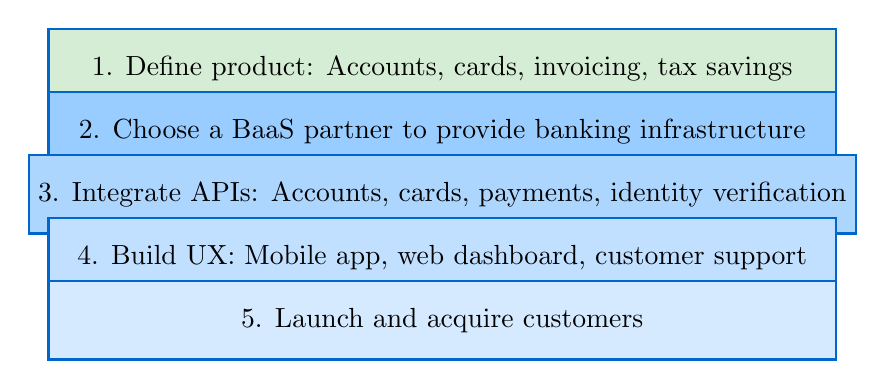
\begin{tikzpicture}[node distance=0.8cm]
\node (step1) [process, fill=dfgreen!20, minimum width=10cm] {1. Define product: Accounts, cards, invoicing, tax savings};
\node (step2) [process, fill=dflightblue, minimum width=10cm, below of=step1] {2. Choose a BaaS partner to provide banking infrastructure};
\node (step3) [process, fill=dflightblue2, minimum width=10cm, below of=step2] {3. Integrate APIs: Accounts, cards, payments, identity verification};
\node (step4) [process, fill=dflightblue3, minimum width=10cm, below of=step3] {4. Build UX: Mobile app, web dashboard, customer support};
\node (step5) [process, fill=dflightblue4, minimum width=10cm, below of=step4] {5. Launch and acquire customers};
\end{tikzpicture}
\end{center}

\vspace{1mm}
\begin{block}{Discussion Questions}
\begin{enumerate}\compactlist
\item What are the biggest risks in this model?
\item What happens if your partner bank faces regulatory problems?
\item How would you differentiate your product from existing neobanks?
\item What data would you need from freelancers that traditional banks do not collect?
\end{enumerate}
\end{block}
\end{frame}

% ============================================================================
% SLIDE 23: EXECUTIVE SUMMARY
% ============================================================================
\begin{frame}{Executive Summary}
\begin{block}{Key Takeaways}
\begin{enumerate}
\item \textbf{APIs unbundled banking}: Any financial service can now be offered separately via standardized interfaces --- breaking the bank monopoly on financial products
\item \textbf{Regulation drives adoption}: In regions where governments mandate open banking, innovation accelerates; in market-driven regions, adoption is slower and more fragmented
\item \textbf{BaaS enables non-banks}: Companies can ``rent'' banking infrastructure (charter, compliance, ledger) instead of building it from scratch, dramatically lowering the barrier to entry
\item \textbf{Embedded finance is the frontier}: Non-financial platforms increasingly offer financial services at the moment of need, making the traditional bank invisible to the end consumer
\item \textbf{Value accrues to the customer interface}: Whoever owns the customer relationship captures the most value in the API economy --- not necessarily whoever holds the banking license
\end{enumerate}
\end{block}
\end{frame}

% ============================================================================
% SLIDE 24: CONCEPT MAP
% ============================================================================
\begin{frame}{Concept Map: The API Economy Ecosystem}
\begin{center}
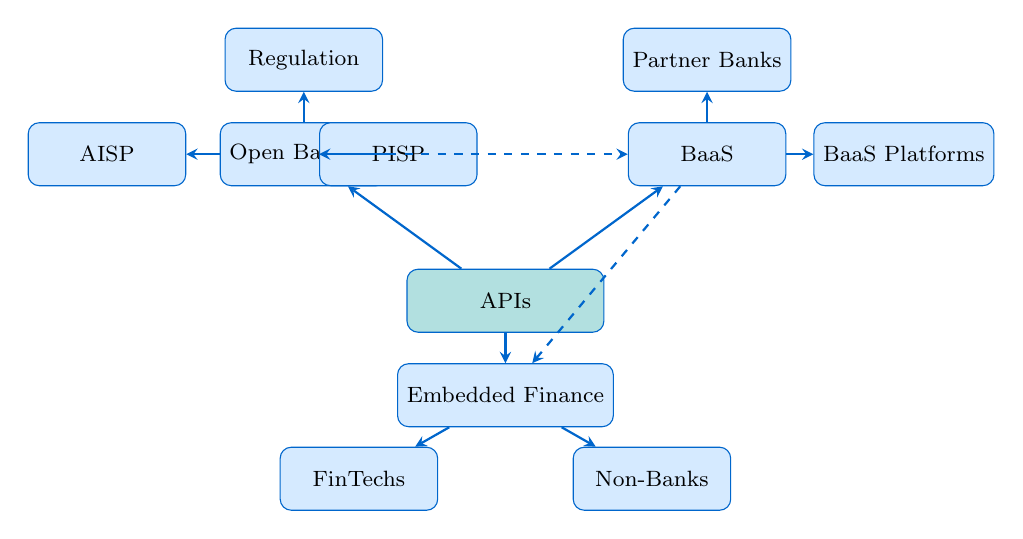
\begin{tikzpicture}[
    node distance=1.5cm,
    concept/.style={rectangle, rounded corners, draw=dfblue, fill=dflightblue4, minimum width=2cm, minimum height=0.8cm, font=\footnotesize, text centered},
    relation/.style={->, >=stealth, dfblue, thick}
]
% Central node
\node (api) [concept, fill=dfteal!30, minimum width=2.5cm] {APIs};

% Top level
\node (openbank) [concept, above left of=api, xshift=-1.5cm, yshift=0.8cm] {Open Banking};
\node (baas) [concept, above right of=api, xshift=1.5cm, yshift=0.8cm] {BaaS};

% Second level
\node (regulation) [concept, above of=openbank, yshift=-0.3cm] {Regulation};
\node (aisp) [concept, left of=openbank, xshift=-1cm] {AISP};
\node (pisp) [concept, right of=openbank, xshift=-0.3cm] {PISP};

\node (partner) [concept, above of=baas, yshift=-0.3cm] {Partner Banks};
\node (platform) [concept, right of=baas, xshift=1cm] {BaaS Platforms};

% Bottom level
\node (embedded) [concept, below of=api, yshift=0.3cm] {Embedded Finance};
\node (fintech) [concept, below left of=embedded, xshift=-0.8cm] {FinTechs};
\node (nonbank) [concept, below right of=embedded, xshift=0.8cm] {Non-Banks};

% Connections
\draw[relation] (api) -- (openbank);
\draw[relation] (api) -- (baas);
\draw[relation] (api) -- (embedded);
\draw[relation] (openbank) -- (regulation);
\draw[relation] (openbank) -- (aisp);
\draw[relation] (openbank) -- (pisp);
\draw[relation] (baas) -- (partner);
\draw[relation] (baas) -- (platform);
\draw[relation] (embedded) -- (fintech);
\draw[relation] (embedded) -- (nonbank);
\draw[relation, dashed] (openbank) -- (baas);
\draw[relation, dashed] (baas) -- (embedded);
\end{tikzpicture}
\end{center}

\vspace{3mm}
\footnotesize{APIs are the technical foundation enabling \textbf{Open Banking} (regulated data access), \textbf{BaaS} (infrastructure rental), and \textbf{Embedded Finance} (integration into non-financial products). Each builds on the previous.}
\end{frame}

% ============================================================================
% SLIDE 25: KEY TERMS
% ============================================================================
\begin{frame}{Key Terms and Definitions}
\begin{description}
\item[API] \textbf{Application Programming Interface} --- A standardized contract allowing software systems to communicate, defining available requests and expected responses.

\item[Open Banking] A regulatory and technical framework requiring banks to share customer data with authorized third parties via secure APIs, with customer consent.

\item[AISP] \textbf{Account Information Service Provider} --- A licensed third party authorized to read and aggregate bank account data (read-only access).

\item[PISP] \textbf{Payment Initiation Service Provider} --- A licensed third party authorized to initiate payments from a user's bank account (write access).

\item[BaaS] \textbf{Banking-as-a-Service} --- A model where licensed banks provide banking infrastructure to non-banks via APIs.

\item[Embedded Finance] Financial services integrated directly into non-financial platforms and customer journeys.

\item[OAuth] An authorization framework allowing third parties to access resources using tokens instead of passwords.
\end{description}
\end{frame}

% ============================================================================
% SLIDE 26: COMMON MISCONCEPTIONS + SELF-ASSESSMENT
% ============================================================================
\begin{frame}{Common Misconceptions and Self-Assessment}
\begin{columns}[T]
\begin{column}{0.48\textwidth}
\textbf{Common Myths:}

\vspace{2mm}
\textcolor{dfred}{\textbf{Myth 1:}} ``Neobanks are banks''\\
\textcolor{dfgreen}{\textbf{Reality:}} Most neobanks are FinTechs partnering with licensed banks. They do not hold a full banking charter themselves.

\vspace{3mm}
\textcolor{dfred}{\textbf{Myth 2:}} ``Open Banking means anyone can see my data''\\
\textcolor{dfgreen}{\textbf{Reality:}} Explicit customer consent is required. You control who accesses what, and can revoke access at any time.

\vspace{3mm}
\textcolor{dfred}{\textbf{Myth 3:}} ``APIs make banking less secure''\\
\textcolor{dfgreen}{\textbf{Reality:}} Proper APIs with token-based authentication are more secure than screen-scraping, which requires sharing passwords.
\end{column}
\begin{column}{0.48\textwidth}
\textbf{Self-Assessment Questions:}

\vspace{2mm}
\begin{enumerate}
\item In your own words, explain the difference between an AISP and a PISP.

\vspace{2mm}
\item Why does a FinTech using BaaS depend on its partner bank's regulatory standing?

\vspace{2mm}
\item What are the advantages of token-based access over password sharing?

\vspace{2mm}
\item If you were building a FinTech, would you apply for your own banking license or use BaaS? Justify your reasoning.
\end{enumerate}
\end{column}
\end{columns}
\end{frame}

% ============================================================================
% SLIDE 27: WHAT'S NEXT + QUESTIONS
% ============================================================================
\begin{frame}{What's Next}
\begin{block}{Coming Up}
\textbf{Topic 2.3: Data-Driven Finance --- Lending, Scoring, and Algorithmic Decisions}
\end{block}

\vspace{3mm}
\textbf{Preview:}
\begin{itemize}
\item How do lenders decide whether to trust you with money they might never see again?
\item Traditional credit scoring vs.\ machine learning approaches
\item Alternative data: what if your everyday financial behavior could help you get a loan?
\item Algorithmic bias: can a ``neutral'' algorithm discriminate?
\item The right to know why you were turned down
\end{itemize}

\vspace{3mm}
\textbf{Connection to this topic:}\\
Open Banking APIs provide the \textbf{data} that powers data-driven finance. Without API access to transaction history, alternative credit scoring would not be possible.

\vspace{5mm}
\centering
{\Large\textbf{Questions?}}

\vspace{3mm}
\textbf{Remember}: Complete Notebook NB03 (Open Banking API Simulation) before the next session.

\bottomnote{Next: Topic 2.3 | Notebook: NB03 --- Open Banking API Simulation}
\end{frame}

\end{document}
